\documentclass[logo,reportComp]{thesis}
\usepackage[cpp,pseudo]{mypackage}

\title{计算机图形学}
\subtitle{作业三:星球旋转}
\school{数据科学与计算机学院}
\author{陈鸿峥}
\classname{17大数据与人工智能}
\stunum{17341015}
\headercontext{计算机图形学作业}
% \lstset{language=python}

\begin{document}

\maketitle

双击打开\verb'planet.exe'即可运行,其他的\verb'glut32.dll'及\verb'glut32.lib'为运行所需的动态/静态库。
四种基本操作如下:
\begin{itemize}
	\item 按d键:小星球正方向自转
	\item 按SHIFT+d键:小星球反方向自转
	\item 按y键:小星球绕大星球正方向公转
	\item 按SHIFT+y键:小星球绕大星球反方向公转
\end{itemize}

设小星球与大星球的距离为$d$,则公转$\theta$弧度后小星球的位置为
\[(x,z)=(d\sin\theta, d\cos\theta)\]
在实际做变换时应注意先进行旋转操作,再进行平移,旋转是绕$y$轴旋转。

同时为更好展示$z$轴上的距离远近,我采用了一线性函数,对小星球的半径进行调整。
当小星球离我们更近时,即在$z$轴正向,则半径最大;反之,离我们越远,其显示半径越小。

实验结果如下图所示。
\begin{figure}[H]
\centering
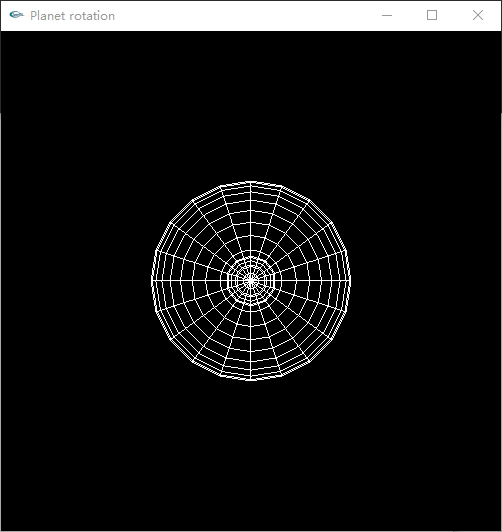
\includegraphics[width=0.6\linewidth]{initial_state.png}
\caption{初始状态}
\end{figure}
\begin{figure}[H]
\centering
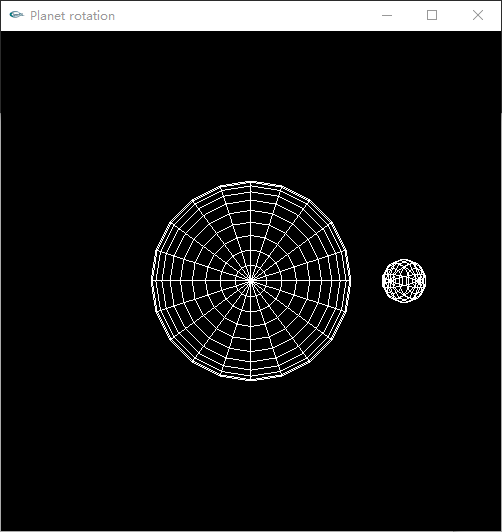
\includegraphics[width=0.6\linewidth]{rotate_state.png}
\caption{旋转后状态}
\end{figure}

实验的代码如下。
\begin{lstlisting}
#include <windows.h>
#include <GL/glut.h>
#include <stdio.h>
#include <math.h>

const double PI = 2*acos(0.0);

int angRot = 0;
int angRevo = 0;
float distance = 0.8;

void myDisplay()
{
    glClear(GL_COLOR_BUFFER_BIT);

    // Big sphere
    glutWireSphere(0.4f, 20, 20);

    float posx = (float) sin((float)angRevo/180*PI) * distance;
    float posz = (float) cos((float)angRevo/180*PI) * distance;

    glPushMatrix(); // only transform smaller one
    // planet revolution
    glTranslatef(posx,0,posz);
    // planet rotation (firstly self rotate)
    glRotatef(angRot,0,1,0);
    // for visualization, the size of the sphere is changed linearly
    glutWireSphere(0.1f*(posz+2*distance)/(3*distance), 8, 8);
    glPopMatrix();

    glFlush();
}

void keyPressed(unsigned char key, int x, int y)
{
    // int mod = glutGetModifiers(); // GLUT_ACTIVE_SHIFT
    printf("Pressed %c!\n", key);
    switch (key){
        case 'd':angRot = (angRot + 10) % 360;break;
        case 'D':angRot = (angRot - 10) % 360;break;
        case 'y':angRevo = (angRevo + 10) % 360;break;
        case 'Y':angRevo = (angRevo - 10) % 360;break;
    }
    myDisplay();
}


int main(int argc, char *argv[])
{
    glutInit(&argc, argv);

    glutInitDisplayMode(GLUT_RGB | GLUT_SINGLE);

    glutInitWindowPosition(100, 100);
    glutInitWindowSize(500, 500);

    glutCreateWindow("Planet rotation");

    glutDisplayFunc(myDisplay);
    glutKeyboardFunc(keyPressed);

    // get into display
    glutMainLoop();

    return 0;
}
\end{lstlisting}

\end{document}

% 1. 使用 OpenGL 实现简易的星球旋转效果,如图 1。程序执行效果见附带压缩包的 EXE 程序(EXE 文件为 Win 程序,使用Mac OS 和 Linux 的同学请参照Win 平台下的执行效果)。
% 功能要求:
% 1. 使用不同尺寸的线框球体(Wire Sphere)表示大小两个星球;
% 2. 使用平移和旋转操作实现小星球自转和绕大星球旋转的功能,键盘事件响应如下: d 和 shift+d: 分别控制小星球正反两个方向的自转; y 和 shift+y: 分别控制小星球绕大星球的正方向和反方向旋转;
% 3. 语言不限,开发平台不限。具体效果展示允许略有差异。
% 4. 要求使用OpenGL 着色器编程方式实现程序。

% 实现提示: 1. 正方向旋转可以通过以下方式求得:d = (d + 10) % 360;反方向则为 d = (d - 10) % 360
% 要求: 1. 作业按百分制评分,没交作业算 0 分;
% 2. 提交代码文件,缺源代码文件的作业成绩减 10 分;
% 3. 提交直接可执行的程序文件或脚本文件,不能运行的程序(含出错,缺 dll 文件等)作业成绩减 10 分;
% 4. 作业文档,包含简要的程序文件说明,运行方法,以及程序运行结果截图,缺文档的作业成绩减 10 分; 5. 发现作业抄袭的本次作业算 0 分。
% 说明: 以小组为单位,组长收齐小组内各位同学的作业,作业用 zip 格式文件打包提交(请尽量减少压缩包文件的体积),以附件方式发送到课程邮箱:cgcourse_homework@qq.com ,若 2 天内没收到回复,请重新发 邮件。
% 请于 10 月 12 日 24:00 前提交。
% 邮件名和压缩包文件名格式如下: 班级 + 学号 + 姓名 + HW3 例:17 计科+16000001+张三+HW3